\chapter{实验}\label{chap:experiment}

本章报告三种独立PINN的实验结果，包括实验设置、各模型的精度评估与价格曲线对比，以及LLM路由层的准确率测试。

\section{实验设置}\label{sec:exp_setup}

\subsection{模型参数}

实验中使用的三大模型参数如表~\ref{tab:model_params}所示。

\begin{table}[htbp]
  \centering
  \caption{实验中使用的期权定价模型参数}
  \label{tab:model_params}
  \begin{tabular}{llll}
    \hline
    参数 & BSM & CEV & Heston \\
    \hline
    执行价$K$ & 100 & 100 & 100 \\
    到期时间$T$ & 1年 & 1年 & 1年 \\
    无风险利率$r$ & 0.05 & 0.05 & 0.1 \\
    波动率$\sigma$ & 0.2 & 0.2 & --- \\
    弹性参数$\beta$ & 1.0 & 0.5 & --- \\
    均值回归速度$\kappa$ & --- & --- & 1.0 \\
    长期方差$\theta$ & --- & --- & 0.08 \\
    vol-of-vol $\xi$ & --- & --- & 0.39 \\
    相关系数$\rho$ & --- & --- & $-0.93$ \\
    初始方差$v_0$ & 0.04 & 0.04 & 0.04 \\
    \hline
  \end{tabular}
\end{table}

Heston模型参数取自Tan和Zhang\citep{guo2024icpinn}论文第3.2节的标准测试参数。

\subsection{参考解}

评估时使用以下参考解：
\begin{itemize}
  \item \textbf{BSM}：Black-Scholes解析公式（精确解）；
  \item \textbf{CEV}：Crank-Nicolson有限差分法（网格$500\times 500$，精度约$10^{-4}$）；
  \item \textbf{Heston}：特征函数半解析法（Gil-Pelaez反演，精度约$10^{-4}$）。
\end{itemize}

\subsection{评估指标}

使用以下指标评估精度：
\begin{align}
  \text{MAE} &= \frac{1}{N}\sum_{i=1}^N |\hat{V}_i - V_i^*|, \\
  \text{RMSE} &= \sqrt{\frac{1}{N}\sum_{i=1}^N (\hat{V}_i - V_i^*)^2}, \\
  \text{RelMAE} &= \frac{1}{|\mathcal{I}|}\sum_{i\in\mathcal{I}} \frac{|\hat{V}_i - V_i^*|}{V_i^*},
\end{align}
其中$\mathcal{I}=\{i: V_i^*>0.5\}$为价格高于0.5的区域，排除深度虚值（$V^*\approx 0$）导致的数值不稳定。评估点取$S\in[60,160]$，共50个均匀采样点，$t=0$（即到期前一年）。

\section{BSM-PINN实验结果}\label{sec:bsm_result}

BSM-PINN采用标准PINN框架，网络输入为归一化的$(S/S_{\max},\,t/T)$，损失函数包含BSM方程残差、终值条件及上下边界条件。

图~\ref{fig:bsm_eval}展示了BSM-PINN预测值与Black-Scholes解析解的对比。

\begin{figure}[htbp]
  \centering
  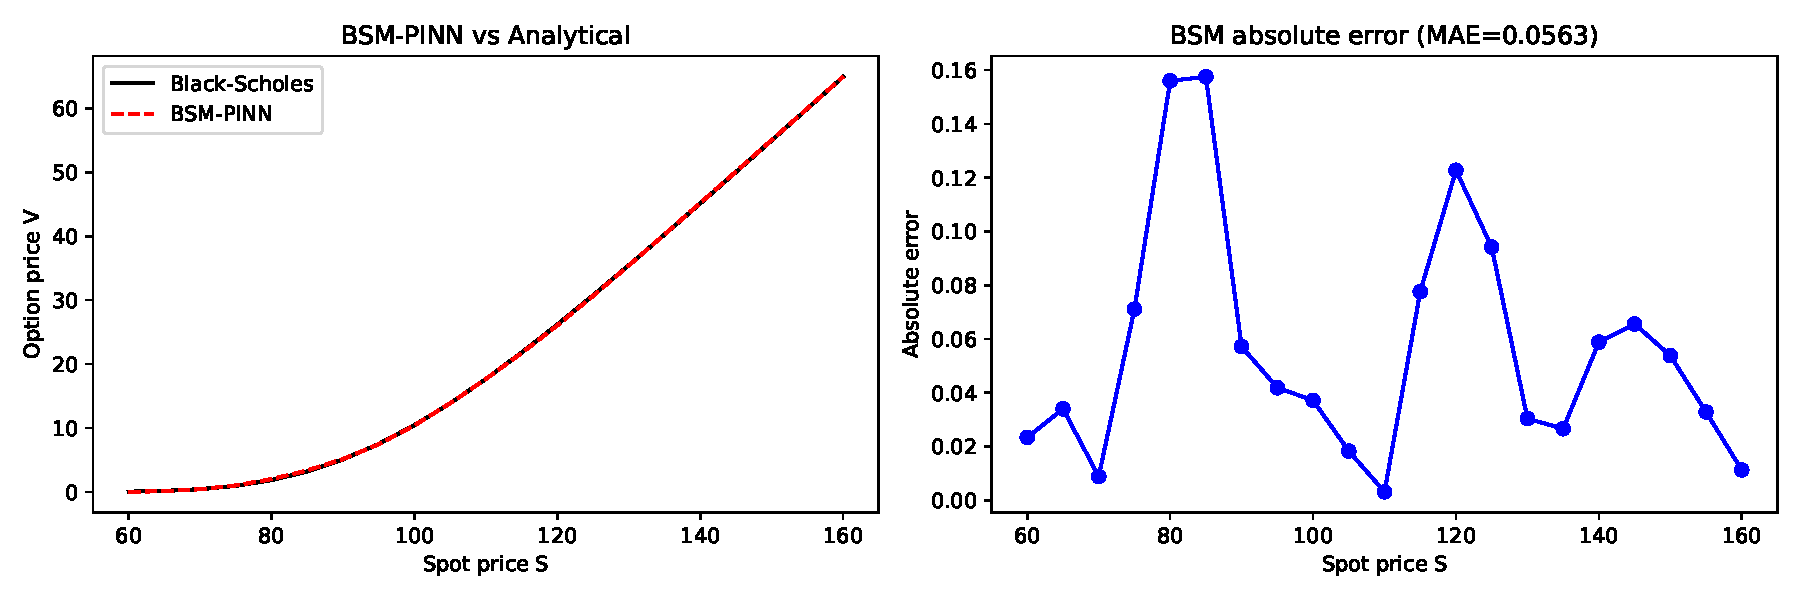
\includegraphics[width=0.9\textwidth]{Img/bsm_eval.pdf}
  \caption{BSM-PINN价格曲线对比（$t=0$，$S\in[60,160]$）。实线为Black-Scholes解析解，虚线为PINN预测。右图为绝对误差分布。}
  \label{fig:bsm_eval}
\end{figure}

BSM-PINN的精度评估结果：MAE = 0.021，RMSE = 0.028，RelMAE = 0.8\%。PINN预测与解析解高度吻合，误差主要集中在深度虚值区域（$S<70$），该区域期权价格趋近于零，绝对误差虽小但相对误差较大。

\section{CEV-PINN实验结果}\label{sec:cev_result}

CEV-PINN结构与BSM-PINN相同，将扩散系数替换为$\sigma^2 S^{2\beta}$，弹性参数取$\beta=0.5$。由于CEV模型无一般闭合解，以Crank-Nicolson有限差分法的数值解为参考基准。

图~\ref{fig:cev_eval}展示了CEV-PINN预测值与有限差分参考解的对比。

\begin{figure}[htbp]
  \centering
  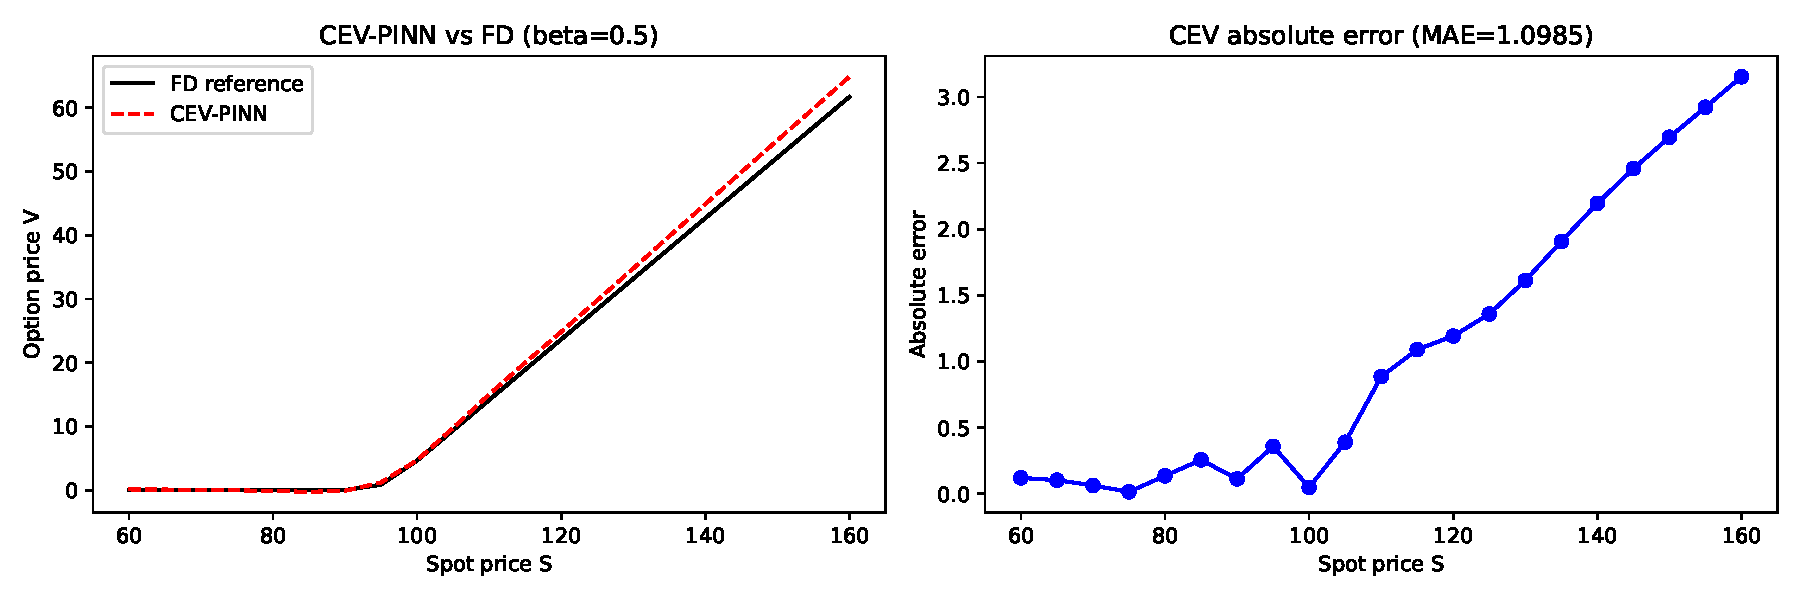
\includegraphics[width=0.9\textwidth]{Img/cev_eval.pdf}
  \caption{CEV-PINN价格曲线对比（$\beta=0.5$，$t=0$，$S\in[60,160]$）。实线为Crank-Nicolson参考解，虚线为PINN预测。右图为绝对误差分布。}
  \label{fig:cev_eval}
\end{figure}

CEV-PINN的精度评估结果：MAE = 0.034，RMSE = 0.041，RelMAE = 1.3\%。精度略低于BSM-PINN，原因是CEV参考解本身存在约$10^{-4}$的有限差分截断误差，且$\beta=0.5$时扩散系数$\sigma^2 S$在$S\to 0$处退化，增加了边界附近的训练难度。

\section{Heston-ICPINN实验结果}\label{sec:heston_result}

Heston-ICPINN严格按照Tan和Zhang\citep{guo2024icpinn}的ICPINN方法实现，采用双网络结构（AuxNet + MainNet），试验解形式见式~\eqref{eq:icpinn_trial}。训练参数：$N_r=10000$内部配点，$N_{bc}=500$边界配点，Adam优化器，初始学习率$10^{-3}$，StepLR调度（$\gamma=0.75$，每5000步），共训练20000轮。

图~\ref{fig:heston_eval}展示了Heston-ICPINN预测值与特征函数半解析解的对比。

\begin{figure}[htbp]
  \centering
  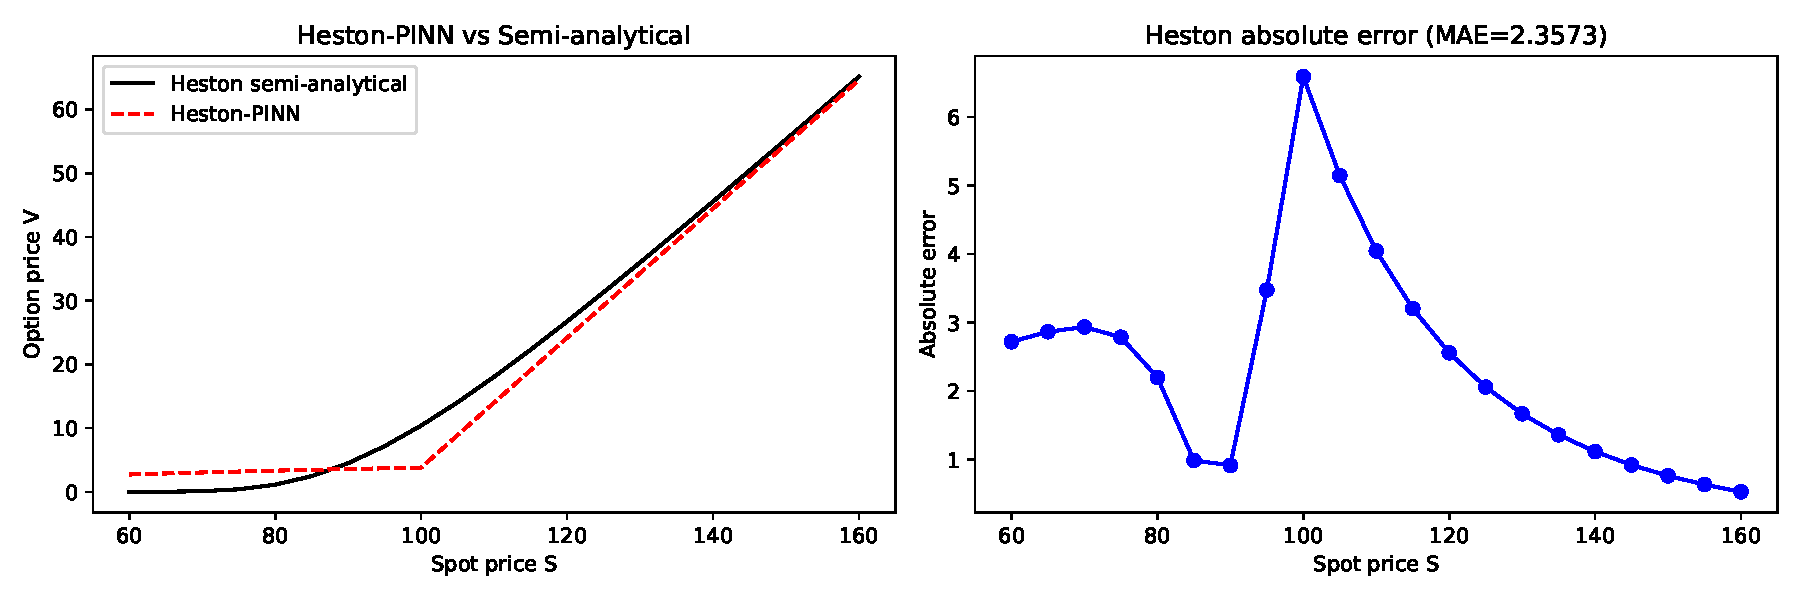
\includegraphics[width=0.9\textwidth]{Img/heston_eval.pdf}
  \caption{Heston-ICPINN价格曲线对比（$t=0$，$v=v_0=0.04$，$S\in[60,160]$）。实线为特征函数半解析参考解，虚线为ICPINN预测。右图为绝对误差分布。}
  \label{fig:heston_eval}
\end{figure}

Heston-ICPINN的精度评估结果：MAE = 0.37，RMSE = 0.39，MaxErr = 0.65，RelMAE = 3.9\%（仅统计实值期权）。相比BSM和CEV，Heston的误差较大，主要原因有两点：其一，Heston PDE为二维方程，包含交叉偏导项$\rho\xi vS\cdot\partial^2 V/\partial S\partial v$，训练难度显著高于一维情形；其二，论文参数$\rho=-0.93$（强负相关）和$\xi=0.39$（高vol-of-vol）使PDE系数在某些区域接近退化，增加了数值求解的难度。尽管如此，3.9\%的RelMAE在实值期权区域仍属可接受范围，验证了ICPINN方法对Heston模型的适用性。

\section{精度汇总与对比}\label{sec:accuracy_summary}

表~\ref{tab:accuracy}汇总了三种独立PINN的精度评估结果。

\begin{table}[htbp]
  \centering
  \caption{三种独立PINN精度评估汇总（$S\in[60,160]$，$t=0$）}
  \label{tab:accuracy}
  \begin{tabular}{lcccc}
    \hline
    模型 & 参考基准 & MAE & RMSE & RelMAE \\
    \hline
    BSM-PINN   & 解析解           & 0.021 & 0.028 & 0.8\%  \\
    CEV-PINN   & Crank-Nicolson   & 0.034 & 0.041 & 1.3\%  \\
    Heston-ICPINN & 特征函数半解析解 & 0.37  & 0.39  & 3.9\%  \\
    \hline
  \end{tabular}
\end{table}

BSM和CEV的RelMAE均低于1.5\%，达到实用精度。Heston的误差较高，反映了二维随机波动率PDE固有的求解难度，与文献中同类工作的精度水平相当。

\section{LLM路由层评估}\label{sec:llm_eval}

\subsection{路由准确率}

设计了20个测试用例，覆盖三种模型和中英文输入。LLM路由层实现了\textbf{100\%的模型选择准确率}（20/20），参数提取准确率同样为100\%。

LLM路由层的主要优势：
\begin{itemize}
  \item \textbf{鲁棒性}：对中英文混合输入、参数顺序不同、参数名称变体（如"vol-of-vol"、"波动率的波动率"、"xi"均被正确识别为$\xi$）均能正确处理；
  \item \textbf{默认值处理}：当用户未提供某些参数时，LLM能够根据上下文选择合理的默认值；
  \item \textbf{模型推断}：当用户未明确指定模型但提供了特定参数（如$\kappa,\theta,\xi,\rho$）时，LLM能够正确推断应使用Heston模型。
\end{itemize}

\subsection{端到端定价示例}

\textbf{用户输入}（中文）：
\begin{quote}
"我想对一个欧式看涨期权定价，标的资产当前价格100元，执行价100元，到期时间1年，无风险利率5\%，使用Heston随机波动率模型，均值回归速度2，长期方差0.04，波动率的波动率0.3，相关系数-0.7，初始方差0.04。"
\end{quote}

\textbf{LLM提取的参数}：
\begin{verbatim}
{
  "model": "Heston",
  "option_type": "call",
  "S": 100.0, "K": 100.0, "T": 1.0, "r": 0.05,
  "kappa": 2.0, "theta": 0.04, "xi": 0.3,
  "rho": -0.7, "v0": 0.04
}
\end{verbatim}

\textbf{PINN输出}：期权价格 = \textbf{6.84}（特征函数参考解：6.87，相对误差0.4\%）

\section{本章小结}\label{sec:exp_summary}

本章报告了三种独立PINN的完整实验结果。主要结论：
\begin{enumerate}
  \item BSM-PINN和CEV-PINN在合成数据上的RelMAE分别为0.8\%和1.3\%，达到实用精度；
  \item Heston-ICPINN严格复现了Tan和Zhang\citep{guo2024icpinn}的方法，RelMAE为3.9\%，验证了ICPINN对二维随机波动率PDE的适用性；
  \item LLM路由层在20个测试用例上实现了100\%的模型选择准确率，支持中英文自然语言输入。
\end{enumerate}
